\documentclass{article}
\usepackage[a4paper,landscape,margin=0.5cm]{geometry}
\pagestyle{empty}

\setlength\parskip{0pt}
\setlength\parindent{0pt}

\usepackage{graphicx, xcolor}
\usepackage{tikz}
\usetikzlibrary{shapes.callouts}
\newcommand{\qrcode}[1]{\middlebox{\includegraphics[height=1.3cm]{#1.png}}}

\newcommand{\textfill}[1]{\resizebox{\linewidth}{!}{#1}}
\usepackage{pbox, lettrine}
\newcommand{\middlebox}[1]{$\vcenter{\hbox{#1}}$}

\newcommand{\ordigibaza}[4]{%
	\begin{minipage}[b][1.1cm]{\linewidth}
		\parbox[c]{11.4cm}{\middlebox{#1} #2}
		{#3\hfill#4}
	\end{minipage}
}

\newcommand{\ordigi}[4]{%
	\ordigibaza{#1}{#2}{#3}{#4}
	\vspace{-0.5\baselineskip}
	\textcolor{gray}{\hrule}
	\vspace{-0.2\baselineskip}
}

\newcommand{\ordigilaston}[4]{%
	\ordigibaza{#1}{#2}{#3}{#4}
	\vspace{-0.7\baselineskip}
}

\newcommand{\cxirkauxi}[1]{\resizebox{1em}{!}{\pbox{100cm}{\begin{tikzpicture}\node[circle, draw, inner sep=0.1cm, line width=2pt] {\resizebox{1em}{!}{#1}};\end{tikzpicture}}}}
\newcommand{\senpaga}{\textsuperscript{\fontspec{Entypo}\hspace{0.1em}♥}}
\newcommand{\paga}{\textsuperscript{\hspace{0.05em}\fontsize{12}{12}\selectfont ₪}\hspace{0.05em}}

\newcommand{\hl}[1]{\textbf{#1}}


\usepackage{fontspec}
\usepackage{bidi}

\setmainfont[Script=Hebrew]{Carmelit}
\newcommand{\url}[1]{\LR{\fontspec{Fontin Sans}#1}}

\begin{document}
\setRL

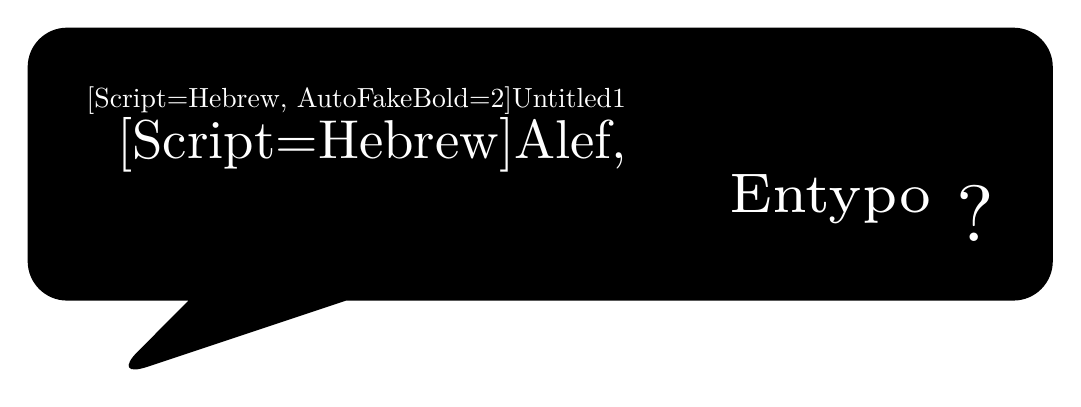
\begin{tikzpicture}
	\node[rectangle callout, fill, callout relative pointer={(-2cm,-1cm)}, callout pointer width=2cm, rounded corners=0.5cm, inner sep=0.75cm, text width=0.95\textwidth] {\color{white}
			\setRL\setmainfont[Script=Hebrew, AutoFakeBold=2]{Untitled1}
			\textfill{{מה{\fontspec[Script=Hebrew]{Alef},} לא חבל {לזרוק חפצים} לפח}}
			\textfill{כשאפשר לתת ולקבל חפצים {בחינם}{\senpaga}?}
	};
\end{tikzpicture}

%\vspace{0.25cm}

\fontsize{29}{29}\selectfont

\ordigi
{{\senpaga}\cxirkauxi{\fontspec{Entypo}🔄}}
{אחת לכמה חודשים,}
{באירועי \hl{מתחלפים בגבעה}}
{\centering\fontsize{20}{20}\selectfont{050-5658042} \fontsize{15}{15}\selectfont{(סמדר)}}

\ordigi
{{\senpaga}\cxirkauxi{\fontspec{Entypo}🔄}}
{שישי הראשון בכל חודש,}
{שוק חופשי ב\hl{זנגביל} ({\fontsize{12}{12}\selectfont\parbox[b]{2.4cm}{\centering בלפור 8, רחביה\\02-5665737}}(}
{~\hfill
	\middlebox{\pbox[t]{100cm}{\fontsize{15}{15}\selectfont\mbox{\url{ginger.org.il}}}}
	\qrcode{zangvil}
}

\ordigi
{{\senpaga}\cxirkauxi{\fontspec{Guttman Hodes}\parbox{1em}{\centering 1\\\small אגורה}}}
{בכל זמן, דרך האינטרנט,}
{באתר \hl{אגורה} {\fontsize{20}{20}\selectfont (לקבל ו/או לתת בחינם)}}%{\fontsize{20}{20}\selectfont (נתינה/קבלה)}}
{~\hfill
	\middlebox{\pbox[t]{100cm}{\fontsize{15}{15}\selectfont\mbox{\url{agora.co.il}}}}
	\qrcode{agora}
}

\ordigi
{{\senpaga}\cxirkauxi{\fontspec{Symbola}🕓}}
{בכל זמן, דרך האינטרנט,}
{באתר \hl{המפקיד} {\fontsize{20}{20}\selectfont (בהשאלה)}}
{~\hfill
	\middlebox{\pbox[t]{100cm}{\fontsize{15}{15}\selectfont\mbox{\url{hamafkid.com}}}}
	\qrcode{hamafkid}
}

\ordigi
%{{\senpaga}\cxirkauxi{\fontspec{Entypo}}}
{{\senpaga}\cxirkauxi{\fontspec{Symbola}👗}}
{בכל זמן אפשר לתת בגדים}
{במכולה ב\hl{מרכז המִחזור} ({\fontsize{12}{12}\selectfont\parbox[b]{3cm}{\centering התחנה הסופית של\\קו~4 במבוא העשׂרה}}(}
{}

\ordigi
{\paga\cxirkauxi{\fontspec{FreeSerif}✌}}
{א׳—ה׳, 9:00—19:00}
{בחנות \hl{כחדש} ({\fontsize{12}{12}\selectfont\parbox[b]{2.4cm}{\centering המרכז המסחרי,\\קומה שניה}}(}
{\fontsize{20}{20}\selectfont{02-5817397}\hspace{1cm}~}

\ordigi
{\paga\cxirkauxi{\fontspec{FreeSerif}✌}}
{בכל זמן, דרך האינטרנט,}
{באתר \hl{יד2}}
{~\hfill
	\middlebox{\pbox[t]{100cm}{\fontsize{15}{15}\selectfont\mbox{\url{yad2.co.il/Yad2}}}}
	\qrcode{yad2}
}

\ordigilaston
{\paga\cxirkauxi{\fontspec{Entypo}📣}}
{}
{כש\hl{אלטע זאכן} עובר… {\fontspec{Symbola}☺}}
{}

\vfill

{
	\fontsize{12}{12}\selectfont
	שימו~{\fontspec{Entypo}♥}: להניח חפצים ליד הפח זאת דרך נהדרת, אלא שמה שלא נלקח מספיק מהר מפונה, וחבל.
	\hfill
	המדבקות הן יוזמה עצמאית מקומית, לא מטעם אף אחד מהנ״ל.
}
 
\vfill

\end{document}
